\chapter{Test automatici generati da LLM}
\label{chap:descrizione-stage-1}
\section{Analisi del dominio applicativo}
Durante la fase di analisi del dominio applicativo si è proceduto a delineare il contesto in cui il progetto si colloca, analizzando il tema e fornendo esempi pratici di utilizzo. Inoltre, si è provveduto a fornire una descrizione esaustiva del meccanismo di \gls{llmse}\glox, tipologia di \gls{llmg} che sta alla base del funzionamento del prodotto.
    \subsection{Analisi del tema}
    Il tema del progetto riguarda la realizzazione di \textit{test} automatici per il codice sorgente, ponendosi come obiettivo la semplificazione del processo di \textit{testing} affidato ai programmatori attraverso l'utilizzo di \glspl{llmg}.
    In particolare, il progetto consiste in uno \textit{script} con il quale vengono estratti i metodi e le classi da testare cercando le relazioni tra di essi. In seguito verrà spigato dettagliatamente come è stato eseguito questo passaggio.
    Lo \textit{script} in questione quindi utilizza predizioni dettate dal \gls{llmg} per generare \textit{test} automatici. Quest'ultimi sono stati successivamente eseguiti e i risultati riportati in grafici per una migliore comprensione.  
    %dopodichè sarà necessario applicare dei filtri per migliorare i risultati ottenuti.
    %Questi filtri sono necessari in quanto, se non applicati, il modello potrebbe generare \textit{test} non validi.

    %descrive il dominio del problema da affrontare:
    %la porzione del mondo reale, rilevante per il sistema\\
    %-> Su cui si devono mantenere informazioni\\
    %-> Concuisideve interagire

    %Dopo la generazione di \textit{test} e il \textit{filtering} di essi, si dovranno quindi salvare nei corrispettivi \textit{file ad hoc}.

    \subsection{Esempi di utilizzo}
    Negli ultimi anni si è registrato un aumento significativo nell'adozione dei \glspl{llmg} per la generazione di testo, con una crescita esponenziale soprattutto nel settore tecnologico.
    In questa sezione si esaminerà il loro utilizzo in ambito di \textit{testing} del codice sorgente.
    In particolare è noto che l'utilizzo di \glspl{llmg} per la generazione di \textit{test} automatici è in grado di ridurre i tempi di \textit{testing} del codice sorgente e migliorare la qualità del codice stesso (Nadia Alshahwan et al.\cite{article:Alshahwan2024AutomatedUT}).
    La capacità di generare test aumenta inoltre la verificabilità di non regressione del codice, ma in questo momento non si è in grado di verificare la presenza di \textit{bug} nel codice senza l'aiuto del programmatore. È chiaro quindi che gli \glspl{llm} in questo periodo storico riescano a fornire solamente un supporto ai programmatori anziché sostituirli.
        %Automatizzazione dei test attraverso llm in modo da aumentare il test coverage dei corner case
        %ridurre bug 
        %ridurre tempo di sviluppo dei test 
    \subsection{\textit{Assured LLMSE}}
    Recentemente nell'ambito del Software Engineering si è assistito ad una crescita elevata dell'utilizzo dell'intelligenza artificiale, volto ad agevolare il programmatore durante lo sviluppo di software.
    Proprio in quest'ambito ci si riferisce a \gls{llmse} per descrivere una qualsiasi tipo di applicazione nella quale il prodotto o i processi software si basano sull'utilizzo di \gls{llm} (Nadia Alshahwan et al.\cite{article:Alshahwan2024AssuredLS}).
    Alla base di questo progetto troviamo quindi un massiccio uso degli \glspl{llm} ed in particolare il progetto in sè vuole fornire uno strumento ai programmatori, che agevoli la scrittura dei \textit{test} attraverso l'utilizzo di \gls{llm}.
    \begin{figure}[!h]
        \centering        
        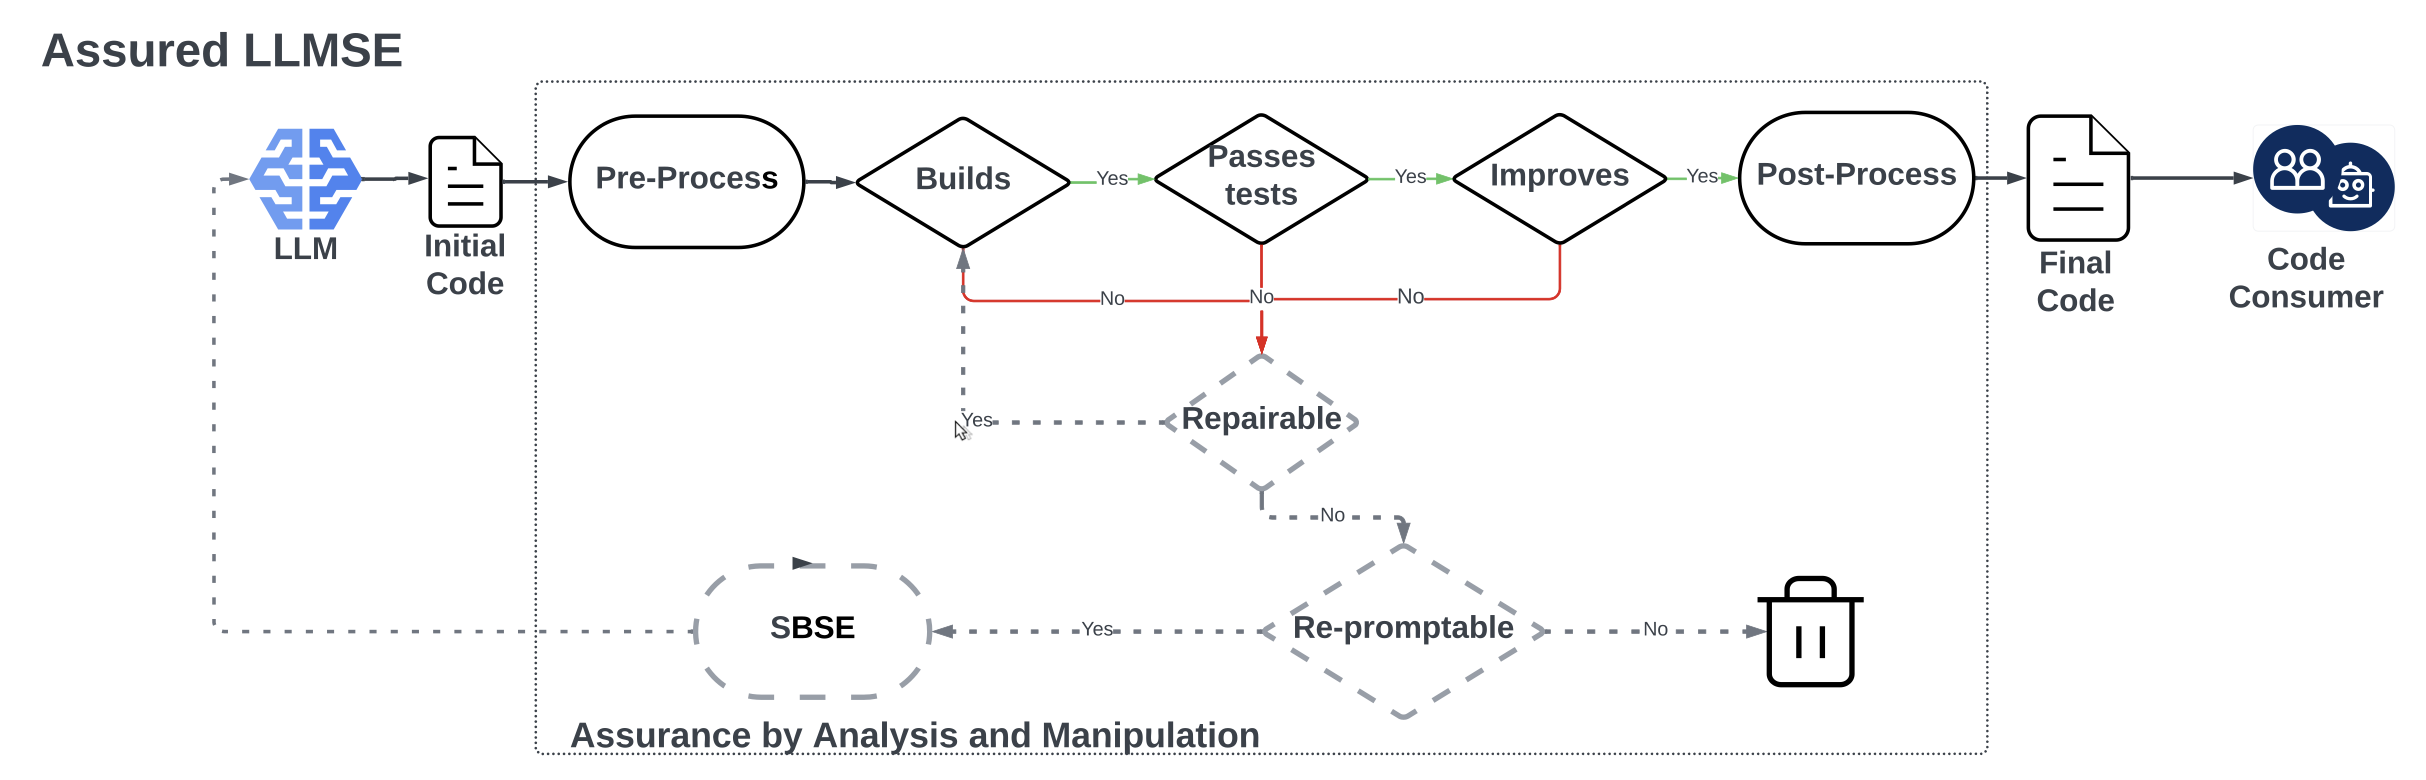
\includegraphics[width=14.5cm]{img/LLMSE.png}
        \caption{Architettura \gls{llmse}\cite{article:Alshahwan2024AssuredLS}}
    \end{figure}
  \\Lo scopo degli \gls{llmse} è quello di applicare una serie di filtri semantici al codice generato in modo tale da poter fornire delle garanzie, come ad esempio l'assenza di allucinazioni.
    Come infatti è visibile in figura 3.1, dopo la generazione della risposta da parte del \gls{llmg}, questa viene pre-processata; si eliminano quindi i vari commenti non soggetti a \textit{test} e si estrae solamente il codice.
    Dopodiché, vengono applicati svariati filtri, tra cui la capacità di essere nello stato di \textit{build}, di essere in stato di accettazione (cioè che l'asserzione di esso sia \textit{true}) ed inoltre che sia in grado di aumentare la \textit{code coverage}.
    È possibile notare che se anche solo uno di questi filtri condizionali non desse risultato positivo, l'intero \textit{test} affronterebbe altri filtri condizionali i quali potrebbero portare alla sua eliminazione.
    Qui di seguito è possibile visionare i filtri che verranno affrontati dal test dopo il fallimento della condizione iniziale.
    \begin{lstlisting}[language=Python]
        def filtering(self, facadeFilter):
            if test.repairable():
                test.repair()
                return facadeFilter.filters(test)
            elif test.re_prompable():
                prompt = test.re_prompt()
                return self.ask(prompt)
            else:
                return test.discard()
    \end{lstlisting}
    
    Nel flusso procedurale, un test scartato viene immediatamente sottoposto al filtro \textit{''Repairable''}. In questo scenario, se è possibile riparare il codice rapidamente senza dover riformulare l'intero prompt, viene effettuata la riparazione e il test riprende il processo di filtraggio. Altrimenti, il test procede con i filtri successivi.
    Nel caso in cui il \textit{Re-prompt} sia possibile, permettendo così di ottimizzare il prompt mediante una riformulazione, il \textit{test} può avanzare alla fase successiva, altrimenti, viene eliminato definitivamente.
    Il \textit{re-prompting} avviene attraverso \textit{Search-based software engineering (SBSE)} che è una tipologia di ottimizzazione del prompt la quale si basa su un algoritmi genetici. La rigenerazione del prompt permette quindi di ricominciare l'interno processo.
    I filtri in questione, nel caso in cui il \textit{test} non fosse approvato, sono filtri opzionali, che verranno omessi durante il processo di sviluppo per ovviare ai costi onerosi derivati.
    Il codice quindi che supera tutti i filtri è un codice che soddisfa i requisiti e può essere passato ad un consumatore, il quale potrebbe essere ad esempio un umano o un altro tool.\newline
        %X cosa sono 
        %X come funzionano 
        %X perchè sono importanti per il progetto 
    \subsubsection{\textit{Offline} ed \textit{Online} LLMSE}
        %distinzione tra off e online
        È importante distinguere \textit{Online} e \textit{Offline} \gls{llmse} in quanto, il primo necessita della risposta dell'\gls{llm} in \textit{real time}, mentre il secondo non pone vincoli temporali.
        Nel contesto dell'\textit{Online} \gls{llmse}, si fa riferimento, ad esempio, alle applicazioni di completamento automatico del codice, come \textit{CoPilot}. Qui, la tempestività della risposta del modello è fondamentale per l'esperienza utente.
        D'altra parte, l'\textit{Offline} \gls{llmse} si riferisce a processi in cui non è necessaria una risposta immediata. Nel caso di \textit{Offline} \gls{llmse}, se il tempo di generazione della risposta dovesse variare, ciò non influirebbe sul funzionamento dell'applicazione stessa. Nello specifico di questo progetto, si utilizzaranno \textit{Offline} \gls{llmse} poichè essi permettono
        di poter applicare i filtri che sono stati precedentemente descritti senza dover preoccuparsi del tempo di risposta.
    \subsubsection{Future applicazioni e miglioramenti} 
        Per quanto riguarda le future applicazioni,
        il perfezionamento dei filtri è sicuramente uno dei maggiori potenziali di sviluppo; in questo modo infatti si riuscirebbero ad ottenere risultati superiori e più adatti alle esigenze.
        Inoltre, anche l'utilizzo di \textit{Genetic Improvement} per perfezionare il \textit{prompt} e \textit{Methauristic algorithm} per ottimizzare le soluzioni candidate potrebbero portare a risultati migliori.
        Il miglioramento del \textit{prompt} è un'area di ricerca molto promettente in quanto, un \textit{prompt} ben formulato è in grado di guidare l'\gls{llm} verso la generazione di test più accurati e corretti. Oltre a ciò, anche l'\textit{in-learning context} è un'area di ricerca che potrebbe portare a risultati significativi. In questo contesto, l'\gls{llm} è in grado di apprendere dai risultati ottenuti e di migliorare le proprie prestazioni nel tempo.
        È possibile quindi ipotizzare che, ponendo maggiore attenzione nel formulare il prompt in modo più accurato, sfruttando algoritmi genetici e applicando le tecniche di \textit{prompt engineering}, si possa ottenere un \gls{llm} più performante e in grado di generare test più accurati e corretti.
        %future applicazioni (?)
        %   -> migliorare filtri
        %   -> Genetic Improvement per migliorare prompt e Methauristic algorithm per migliorare candidate solutions
        %   -> prompt engineering
        %   -> in-learning context
\section{Analisi dei requisiti}
    \subsection{Analisi preventiva dei rischi}
    Durante la fase di analisi dei rischi sono stati individuate le possibili criticità che potranno essere riscontrate durante il progetto.
    Si è quindi proceduto a elaborare delle possibili soluzioni per far fronte a tali rischi.

    \begin{risk}{Mancanza di materiale informativo}
        \riskdescription{Trattandosi di una novità nel settore e in fase di crescita, la possibile assenza di materiale informativo relativo all'argomento stesso potrebbe rallentare il processo di apprendimento}
        \risksolution{coinvolgimento del responsabile a capo del progetto relativo}
        \label{risk:data-absence} 
    \end{risk}

    \subsection{Requisiti e obiettivi}

    \begin{center}
        \rowcolors{1}{}{tableGray}
        \begin{longtable}{|p{2.25cm}|p{7.75cm}|p{2.25cm}|}
        \hline
        \multicolumn{1}{|c|}{\textbf{Obiettivo}} & \multicolumn{1}{c|}{\textbf{Descrizione}}\\ 
        \hline 
        \endfirsthead
        \multicolumn{3}{c}%
        {{\bfseries \tablename\ \thetable{} -- Continuo della tabella}}\\
        \hline
        \multicolumn{1}{|c|}{\textbf{Obiettivo}} & \multicolumn{1}{c|}{Descrizione}\\ \hline 
        \endhead
        \hline
        \multicolumn{3}{|r|}{{Continua nella prossima pagina...}}\\
        \hline
        \endfoot
        \endlastfoot 
        OB 1 & Realizzazione di smoke \textit{test} in Python generati da codice reale. \\
        \hline
        OB 2 & Realizzazione di decorazioni assert per funzioni. \\
        \hline
        OB 3 & Realizzazione di \textit{test} a partire da codice commentato. \\
        \hiderowcolors
        \caption{Requisiti primo macroperiodo.}
        \label{tab:requisiti_obbiettivi}
        \end{longtable}
    \end{center}


\newpage
\section{Sviluppo del prodotto}
    A seguito dello studio del dominio e delle opportunità, vi è stata la progettazione e lo sviluppo del prodotto. 
    Questo capitolo si propone di offrire un'esauriente panoramica sul processo di sviluppo, esaminando nel dettaglio le tappe fondamentali che sono state affrontate.
    In particolare, ci si concentrerà sull'analisi dello \textit{script} realizzato per l'estrazione e la generazione dei \textit{test}, una fase cruciale che ha richiesto un'accurata progettazione e implementazione.
    Verranno poi descritti i risultati ottenuti attraverso un'analisi dettagliata, evidenziando le sfide superate e i successi raggiunti nel corso del processo di sviluppo.
    
    \subsection{\textit{Script}}
    Lo \textit{script} generato permette di fare il parsing di un intero progetto salvando dati chiave all’interno di un \textit{database} \textit{SQlite}. 
    Questo procedimento permette all'\gls{llm} di riuscire a trovare le relazioni all’interno dei dati. 
    Dopo il processo di \textit{parsing} è possibile generare i \textit{test} attraverso l'\gls{llm}. Utilizzando infatti i comandi –-genTestClass e\\ 
    –-genTestMethod è possibile generare i \textit{test} per una classe o per un metodo specifico.
    Il seguente \textit{script} può quindi essere azionato attraverso linea di comando utilizzando vari comandi:
    \begin{itemize}
        \item “python3 –-parseProj nameProject” : si farà solamente il parsing di tutti i file all’interno del progetto.
        \item “python3 –-genTestClass Class\_Name Method\_Name: attraverso questo comando è possibile generare i \textit{test} per un particolare metodo all’interno della classe specificata.
        \item “python3 --genTestMethod Class\_Name: attraverso questo comando è possibile generare i \textit{test} per la singola classe.
    \end{itemize}
    In figura 3.2 viene descritto come sono stati realizzati.\\
    \begin{figure}[!h]
        \centering        
        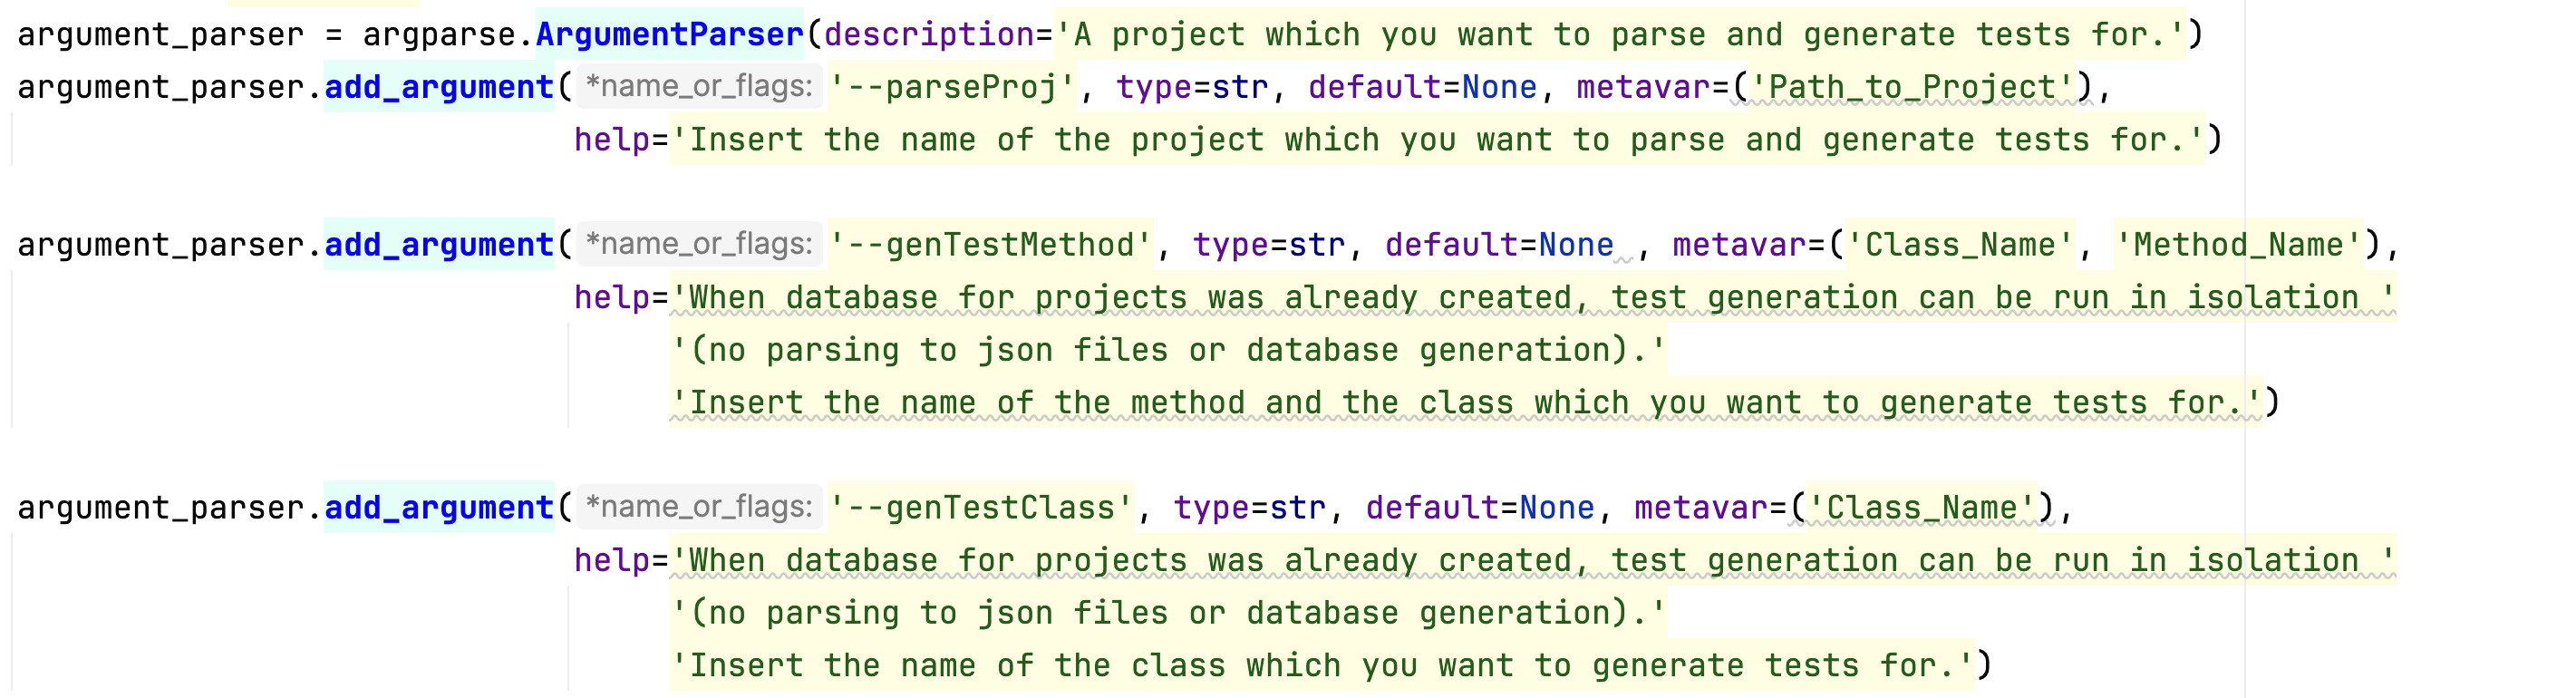
\includegraphics[width=14.5cm]{img/script argument.png}
        \caption{Comandi \textit{script}}
    \end{figure}\newline

    \subsubsection{\textit{Parsing del linguaggio}}
    Inizialmente lo \textit{script} richiede di eseguire l'analisi del progetto, focalizzandosi principalmente sull'estrazione di ogni file con estensione "\textit{.py}"
    e sulla categorizzazione di ciascuna istruzione all'interno di un nodo dell'albero di parsing. Tale processo è indispensabile poichè altrimenti, sarebbe 
    impossibile delineare le relazioni esistenti tra i vari metodi e le classi.
    Una volta estratte e categorizzate tutte le istruzioni all'interno dei nodi dell'albero, vengono recuperate le firme dei metodi e delle classi. 
    Queste informazioni vengono quindi archiviate nel database SQLite insieme ai \textit{related method}, ovvero i metodi chiamati all'interno di altri metodi. 
    Tale approccio consente di identificare le relazioni intrinseche presenti nel progetto e di ottenere risultati più accurati.
    L'idea di base può essere confermata attraverso i dati in figura 3.3.
    \begin{figure}[htp]
        \centering        
        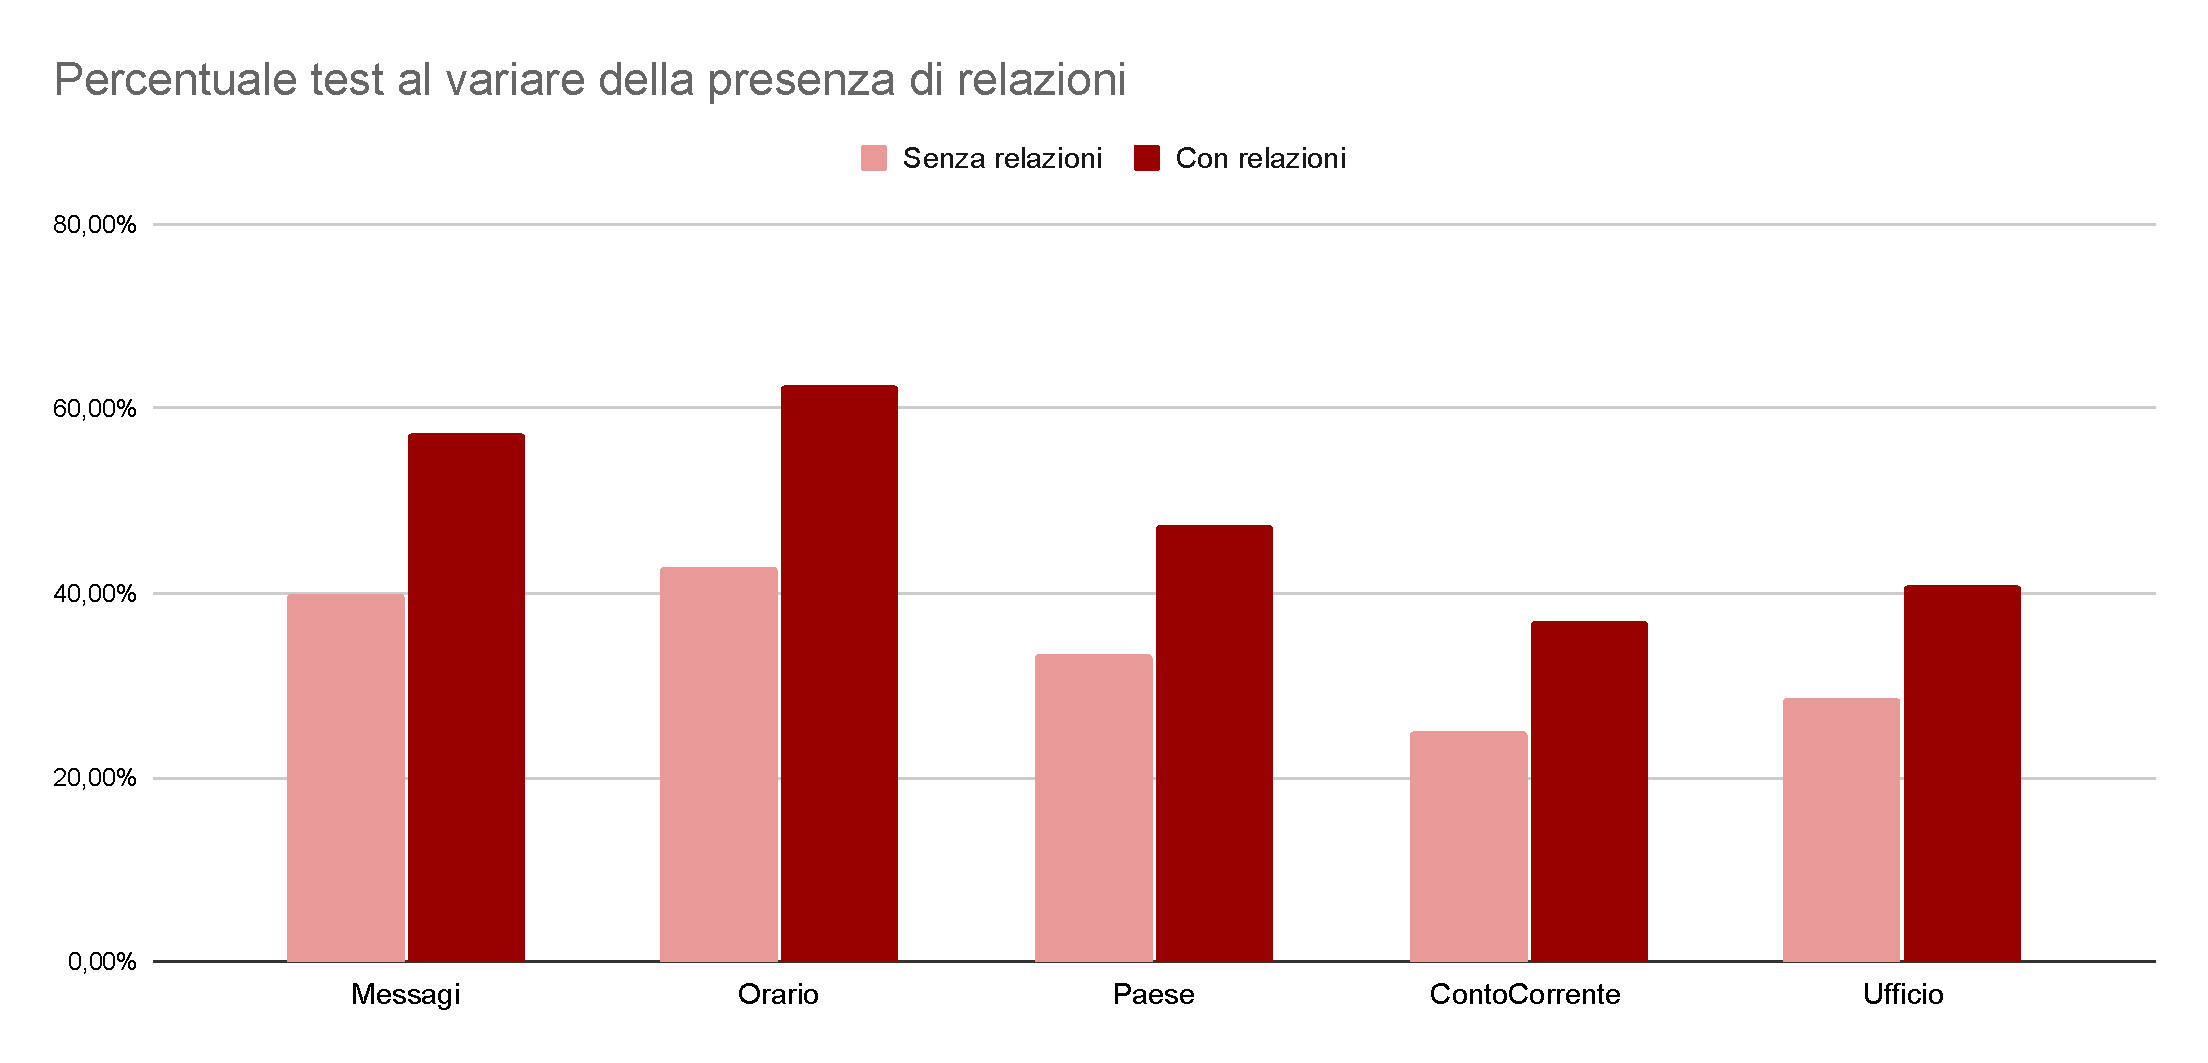
\includegraphics[width=14.5cm]{img/Percentuale test al variare della presenza di relazioni.pdf}
        \caption{Apporto valoriale delle relazioni tra classi nei test}
    \end{figure}\newline
     Il grafico illustra la differenza tra i \textit{test} generati senza inserire nel \textit{prompt} le classi con relazioni con quella da testare e quelli 
    con l'aggiunta di classi inserite nel \textit{prompt}. È chiaramente visibile sia che la quantità di \textit{test} generati nel secondo caso è maggiore sia che il numero di \textit{test} che passano è notevolmente più alto.
    In particolare, la generazione di \textit{test}, includendo anche le classi in relazione, ha generato mediamente il 15\% in più di \textit{test} corretti.
    Un quesito però che ricorre frequentemente nello sviluppo dei \gls{llm} è la \textit{large context window}, in particolare l'aggiunta dei \textit{related\_method} e delle \textit{related\_class} potrebbe portare ad alcuni problemi, tra cui la moltitudine di dati da processare e l'\textit{information overload}.
     L'\textit{information overload} potrebbe portare a un maggior \textit{focus} sugli \textit{edges} del \textit{context} se questo fosse troppo ampio, e ciò porterebbe a perdere il \textit{focus} sulle parti più importanti della domanda. È stato quindi di fondamentale importanza affrontare questa sfida durante lo sviluppo per capire la quantità di metodi e classi relazionate alla classe della quali si sarebbe dovuto generare i \textit{tests}.
    La seconda problematica riscontrata durante il parsing riguarda la tipizzazione dei linguaggi, in particolar modo l'analisi sintattica è stata senza dubbio un'attività dispendiosa in termini di tempo ed energia, poichè il linguaggio di programmazione Python, essendo non tipizzato, non presenta una distinzione chiara tra le istruzioni. In particolare, l'istanziazione di un oggetto è trattata come un'assegnazione in mancanza di una parola chiave specifica. Pertanto, è plausibile ipotizzare che l'analisi sintattica in Java, un linguaggio tipizzato con restrizioni più rigorose, sia più agevole e conduca a risultati più accurati.
    % generazione script per scegliere classi da testare ed eseguire i test
    % generazione di filtri per migliorare i risultati e renderli adatti
    % scelgo progetto e classi, attraverso le relazioni tra classi e metodi, genero test
    % deduciamo che è importante trovare relazioni tra le classi, in linguaggi come Java è più semplice effettuare
    % parsing, in linguaggi privi di semantica invece è difficile andare a trovare queste relazioni e fare parsing.
    % è quindi anche più complesso effettuare il testing di queste classi poichè è difficile a monte trovare 
    % relazioni tra le classi e i metodi.
    
    \subsubsection{Generazione dei \textit{test}}
    Una volta completato il parsing del progetto, lo \textit{script} può essere avviato attraverso i comandi sopra citati.
    In particolare, il comando “python3 --genTestClass Class\_Name” permette di generare i \textit{test} per una particolare classe all'interno del progetto.
    Quando si esegue questo comando, lo \textit{script} recupera la classe scelta all'interno del database e genera i test di unità per i metodi della classe stessa.
    Il secondo comando “python3 --genTestMethod Class\_Name Method\_Name” invece consente di generare i \textit{test} per un metodo specifico all'interno della classe.
    Come nel caso precedente, lo \textit{script} recupera la classe e il metodo scelti all'interno del database e genera i \textit{test} di unità per il metodo selezionato.
    La generazione dei \textit{test} può essere effettuata attraverso l'utilizzo della \textit{Hugging Face Inference API} o tramite un \textit{server} locale. 
    L'impiego di \textit{Hugging Face} consente l'utilizzo di modelli di dimensioni considerevoli, come ad esempio \textit{Llama3 70b}, i quali sono in grado di produrre test più accurati e corretti. Tuttavia, ciò comporta un rallentamento della velocità di inferenza ed un aumento dei costi. 
    Dall'altro lato, l'utilizzo di un \textit{server} locale offre una maggiore velocità di inferenza, ma l'impiego di modelli di dimensioni ridotte, come ad esempio \textit{Chat Qwen 1.5 1b q4}.
    % generazione di test attraverso llm 

    \subsection{\textit{Benchmarks}}
    % benchmarking degli LLM
    % generazione di test attraverso OpenAI e linguaggi invece addestrati su codice
    Dopo lo sviluppo dello \textit{script}, vi è stato un periodo di \textit{test} fondamentale per due scopi. La prima motivazione è legata all'ottimizzazione del \textit{prompt} per migliorare i risultati.  Infatti, andando ad ottimizzare il prompt in modo tale da poter produrre domande più specifiche e maggiormente comprensibili all'\gls{llm},  si possono ottentere \textit{test} più accurati e corretti. 
    La seconda motivazione riguarda il confronto tra i vari \gls{llm} utilizzati.
    Era necessario capire se l'utilizzo di \gls{llm} addestrati su codice sorgente fosse più efficace rispetto a quelli addestrati su testo generico; oltre a ciò, era di fondamentale importanza comprendere quale fosse l'\gls{llm} più adatto per il progetto.
    Ricordando che uno degli scopi principali del progetto è la ricerca dell’\gls{llm} più adeguato alle esigenze e alle possibilità di Zucchetti, 
    inizialmente si è proceduto alla ricerca della temperatura adeguata affinché il modello riuscisse a produrre risultati attendibili evitando 
    l’utilizzo di \gls{llm} molto pesanti. I dati ottenuti sono raffigurati nella figura 3.4 sottostante.\newpage
    \begin{figure}[!h]
        \centering        
        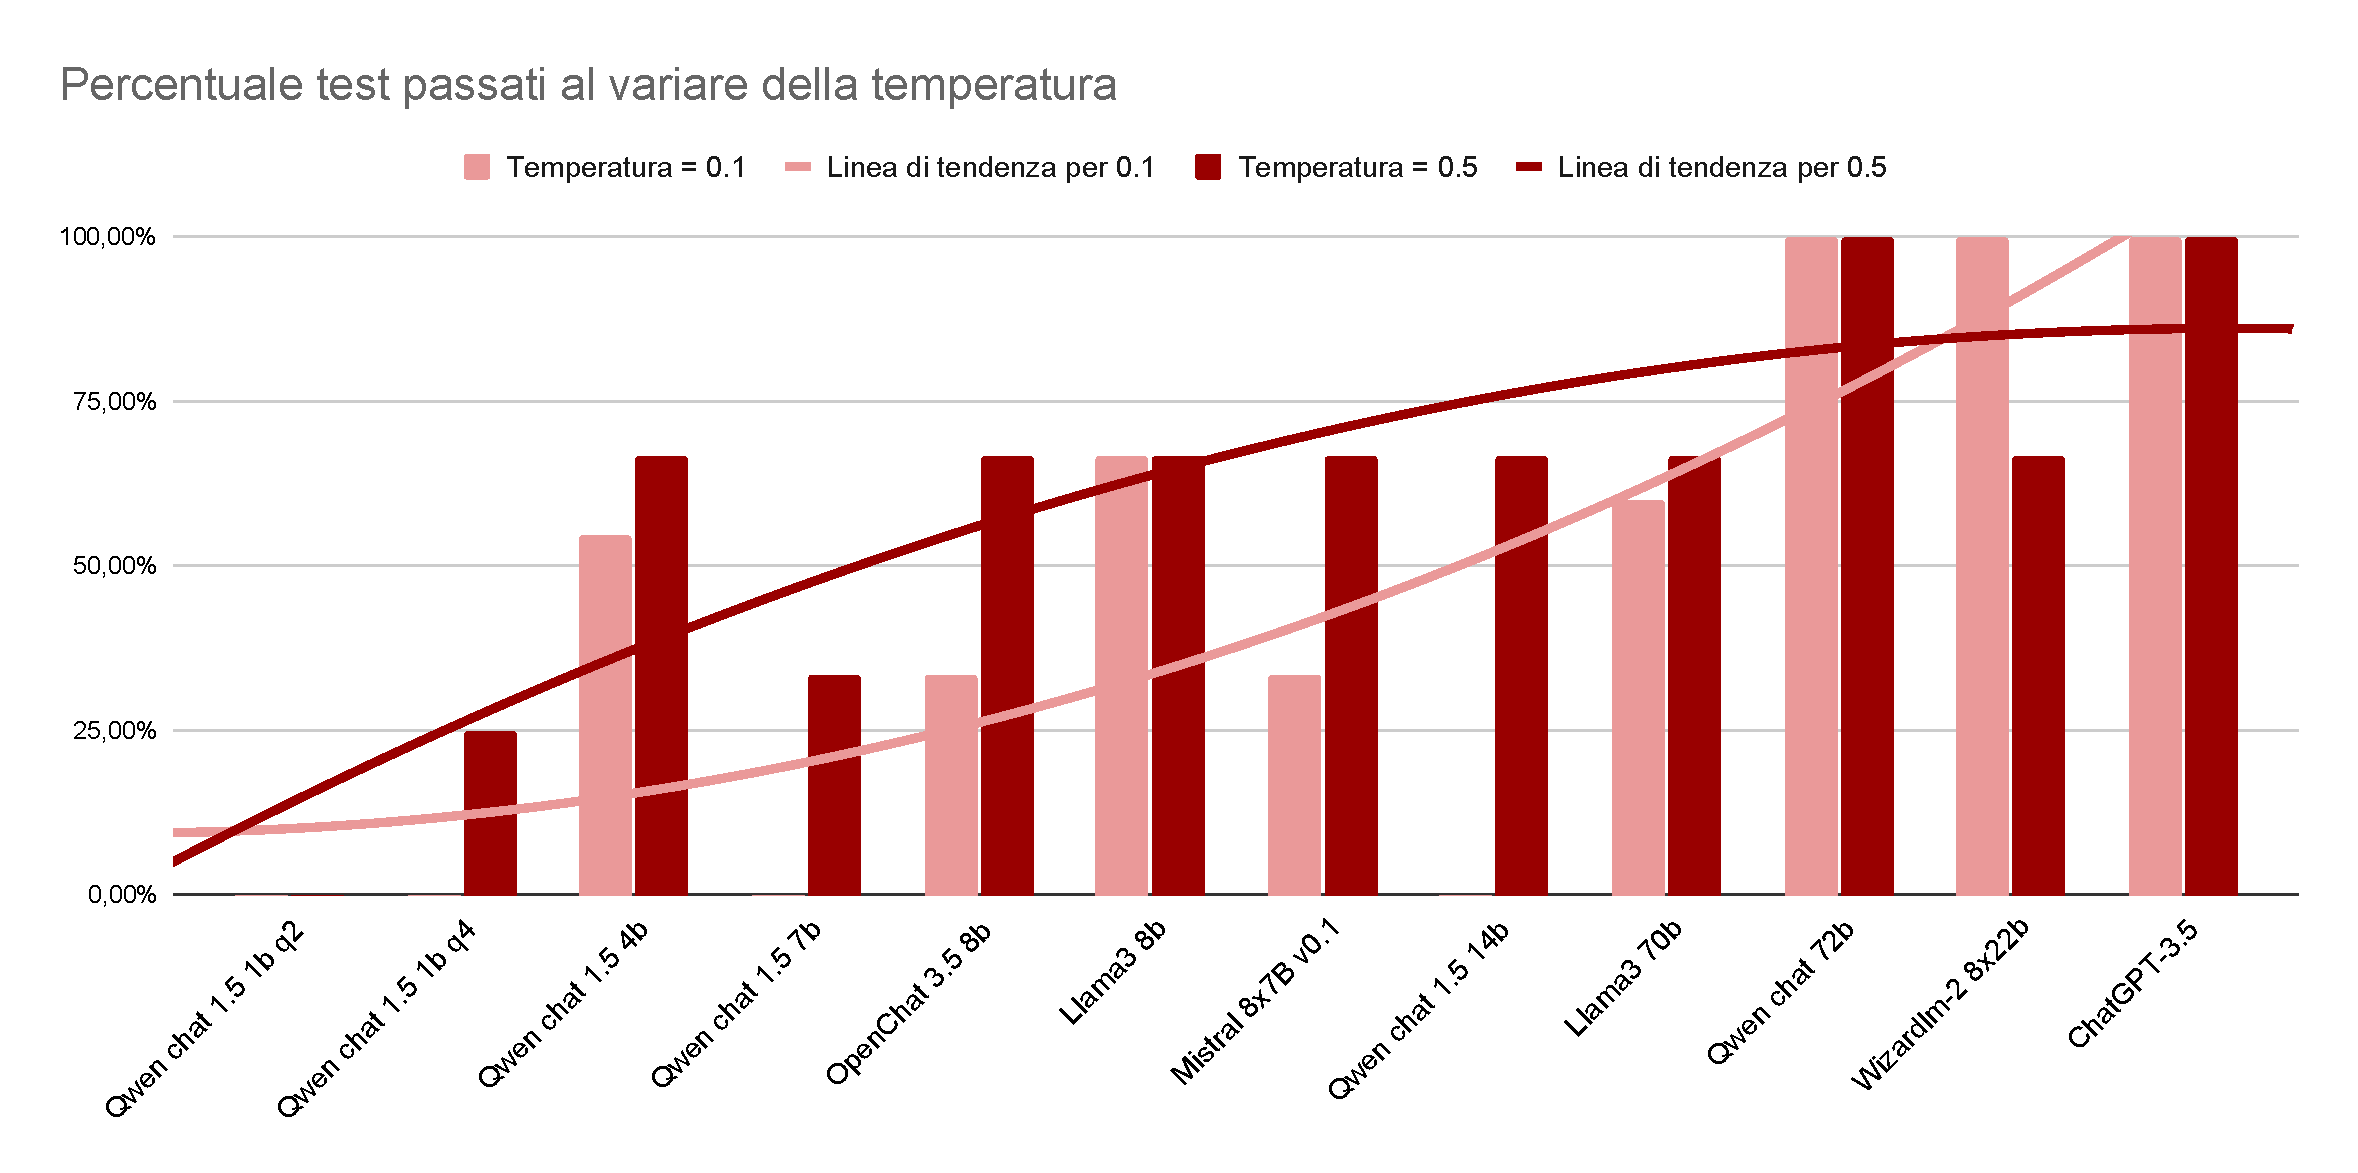
\includegraphics[width=14.5cm]{img/Percentuale test passati al variare della temperatura.pdf}
        \caption{Test generati attraverso temperature diverse}
    \end{figure}
    \\È noto che aumentando la temperatura, un \gls{llmg} produce dati meno deterministici e offre la possibilità di ottenere risultati più diversificati.
    Questo è particolarmente evidente nel caso di modelli con al massimo 14 miliardi di parametri. 
    In tal caso, diventa chiaro che mantenere un elevato grado di determinismo non comporta vantaggi significativi, 
    poiché il numero di parametri è minore e, di conseguenza, anche le conoscenze del modello sono limitate. Nel caso invece 
    di modelli più grandi, questo vantaggio non si percepisce, ed anzi, in un caso in particolare, la sua capacità di generazione di \textit{test} corretti diminuisce.
    Il secondo \textit{test} di rilievo riguarda l'impiego di codice commentato (figura 3.5). Si è ipotizzato che fornendo maggiori dettagli all'\gls{llm}, 
    anche se in forma di linguaggio naturale, il modello potesse generare \textit{test} più efficaci. I risultati ottenuti sono indubbiamente 
    i più significativi, poiché l'aumento delle informazioni nei modelli più piccoli porta quasi sempre a risultati superiori rispetto 
    a quelli ottenuti con modelli più grandi. Inoltre, gli stessi modelli hanno prestazioni migliori su prompt con commenti rispetto a
     quelli privi di essi. È possibile pertanto supporre che ciò sia dovuto al fatto che, avendo meno informazioni a disposizione, l'incremento di esse 
     attraverso il testo aggiuntivo possa notevolmente migliorare le capacità del modello.
    \begin{figure}[htp]
        \centering        
        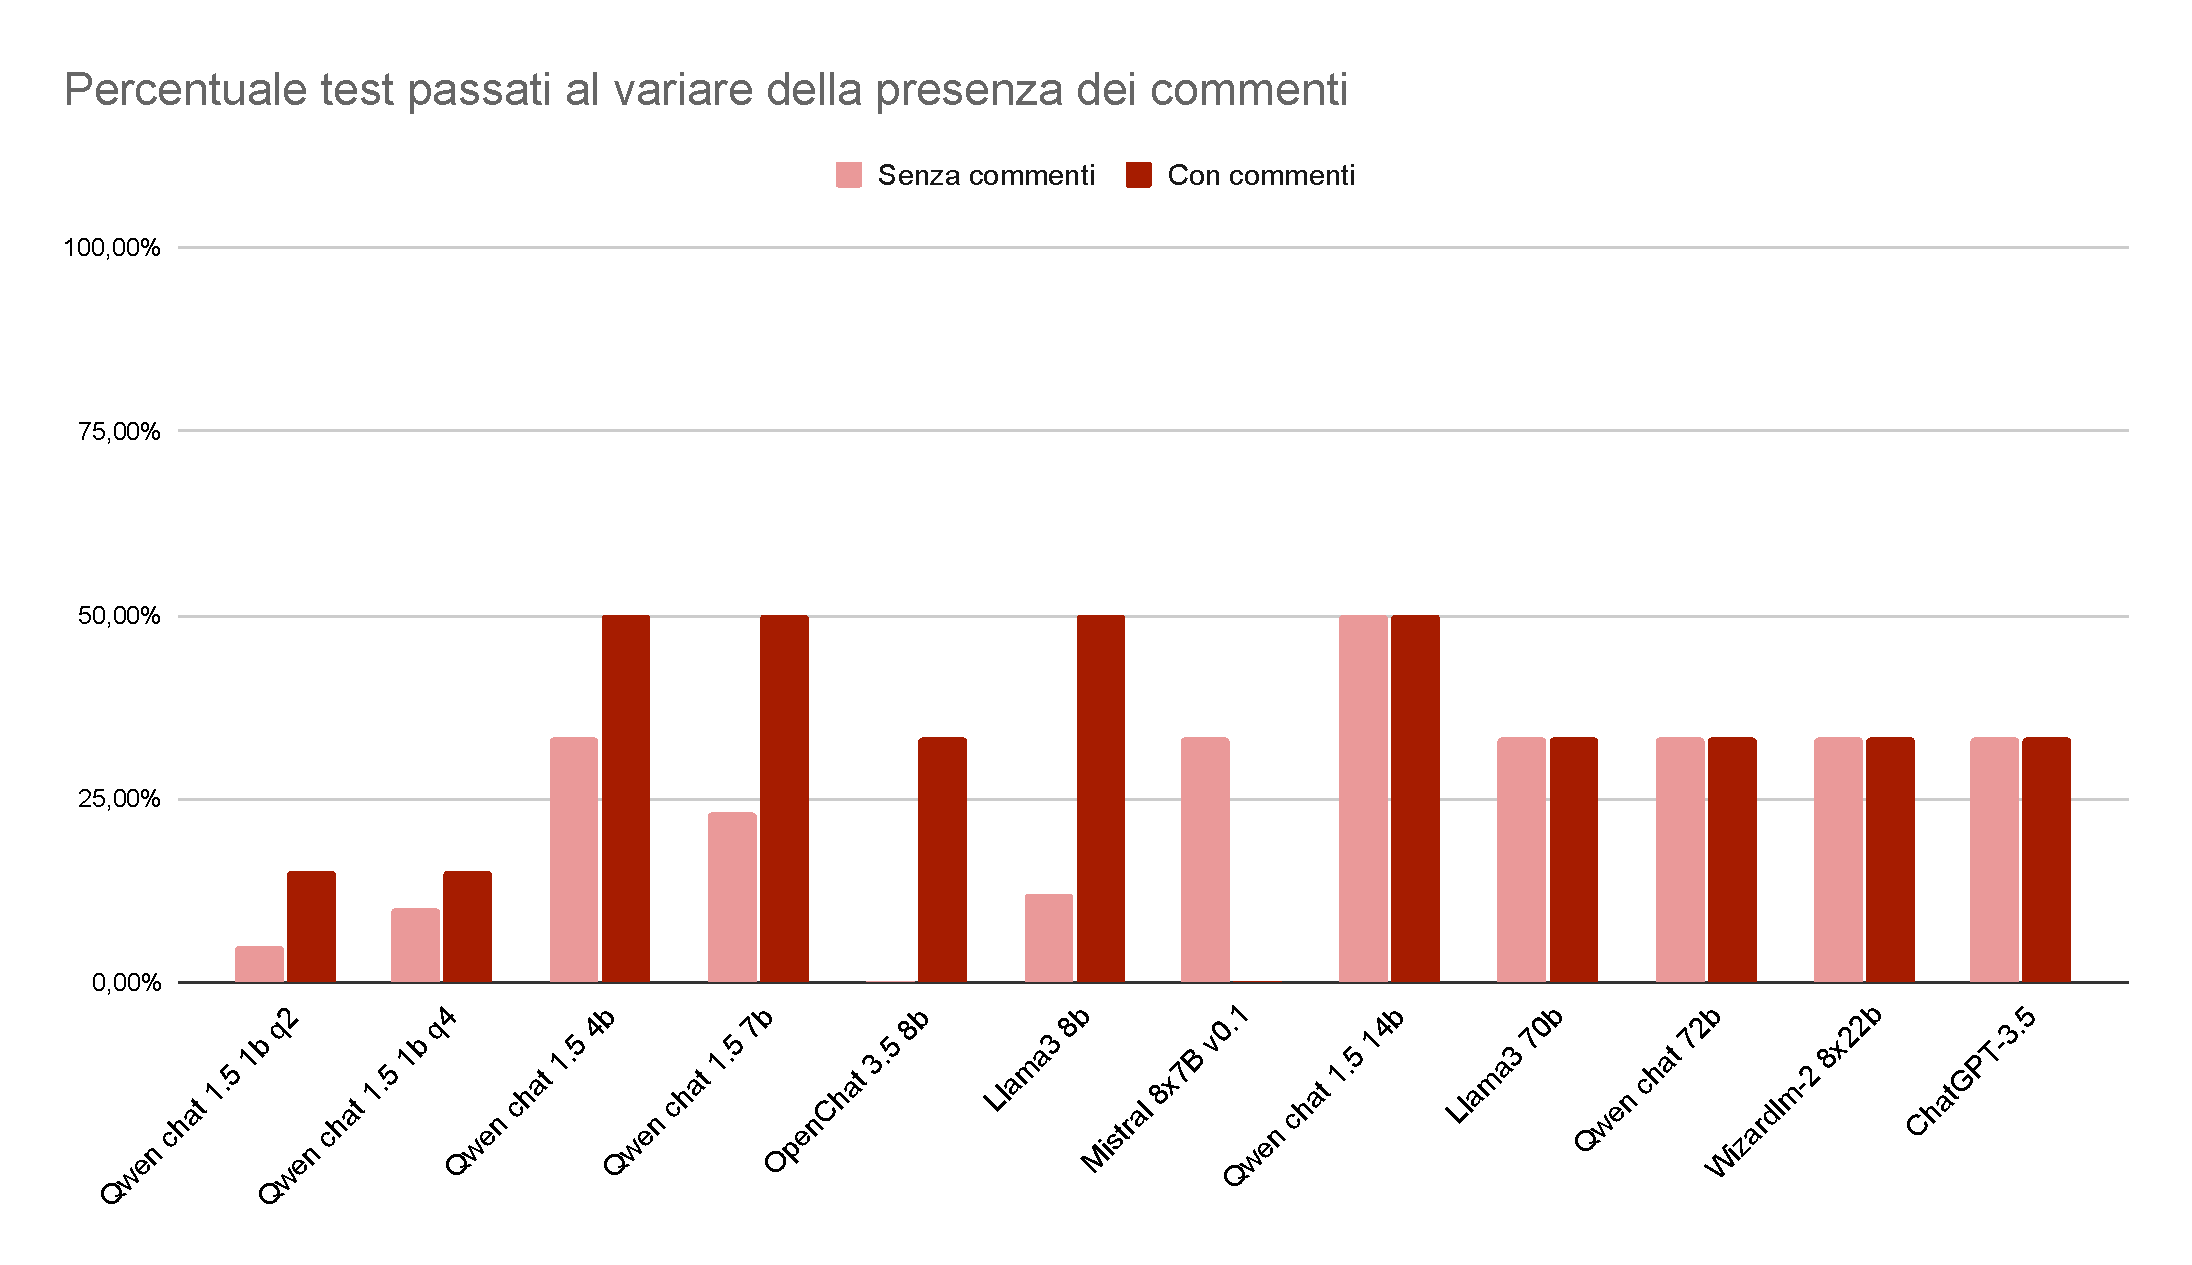
\includegraphics[width=14.5cm]{img/Percentuale test passati al variare della presenza dei commenti.pdf}
        \caption{Test generati attraverso temperature diverse}
    \end{figure}\newpage   
 Dopo queste rilevazioni, si è deciso di confrontare la capacità di generazione di test su codice scritto in inglese e in italiano. L'ipotesi di partenza era che la quantità di dati in italiano fosse inferiore rispetto a quella in inglese e si voleva verificare se questa differenza avrebbe influito in modo significativo sui risultati ottenuti, determinando se l'ipotesi fosse fondata.
    I risultati ottenuti sono raffigurati in figura 3.6 e figura 3.7.
    \begin{figure}[htp]
        \centering        
        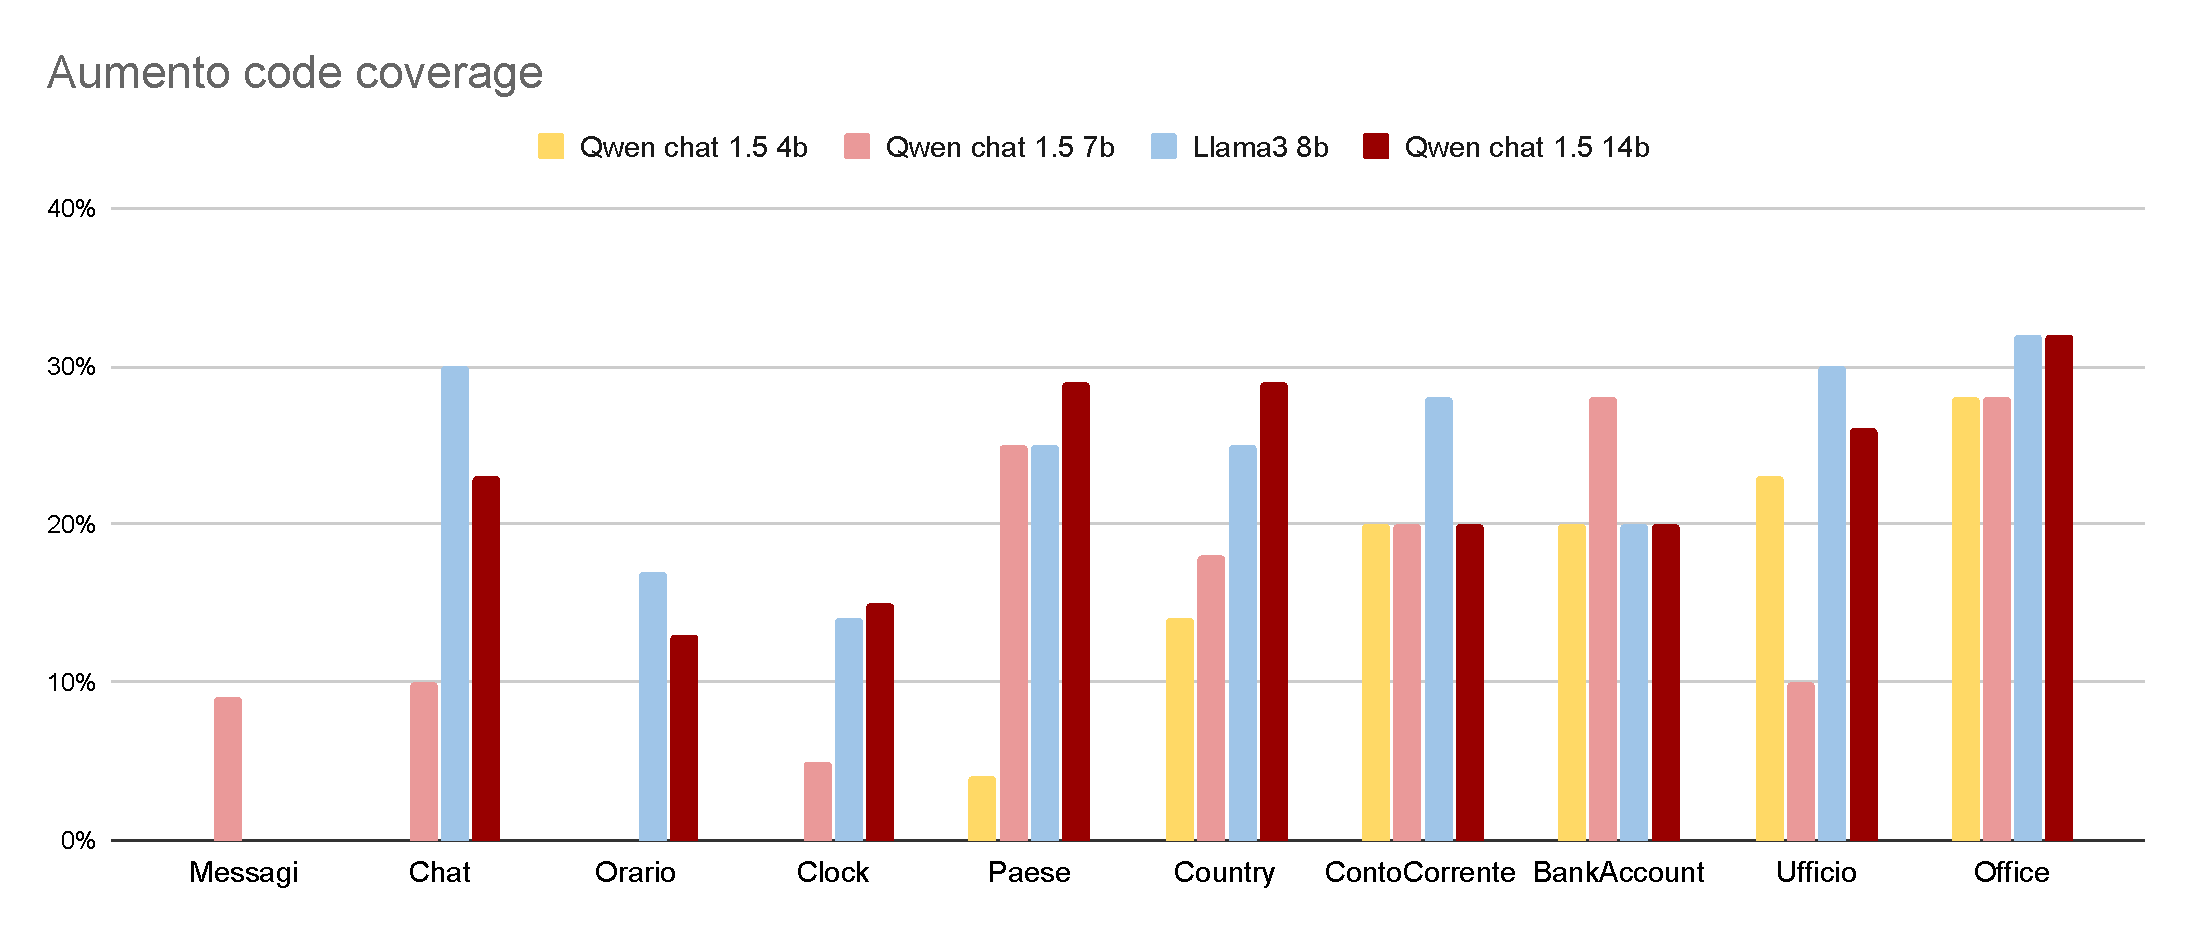
\includegraphics[width=14.5cm]{img/Aumento code coverage.pdf}
        \caption{Aumenti del code coverage al variare della lingua e dei modelli}
    \end{figure}\newline 
    In figura 3.6  è sorprendente notare che in molti casi la quantità di \textit{code coverage} aumentata è molto simile tra \textit{llama 8b} e \textit{Qwen chat 14b}.
    In questi test quindi, sebbene \textit{Qwen chat} sia addestrato su una mole di dati maggiore di \textit{llama}, i risultati sono molto simili.
    \begin{figure}[htp]
        \centering        
        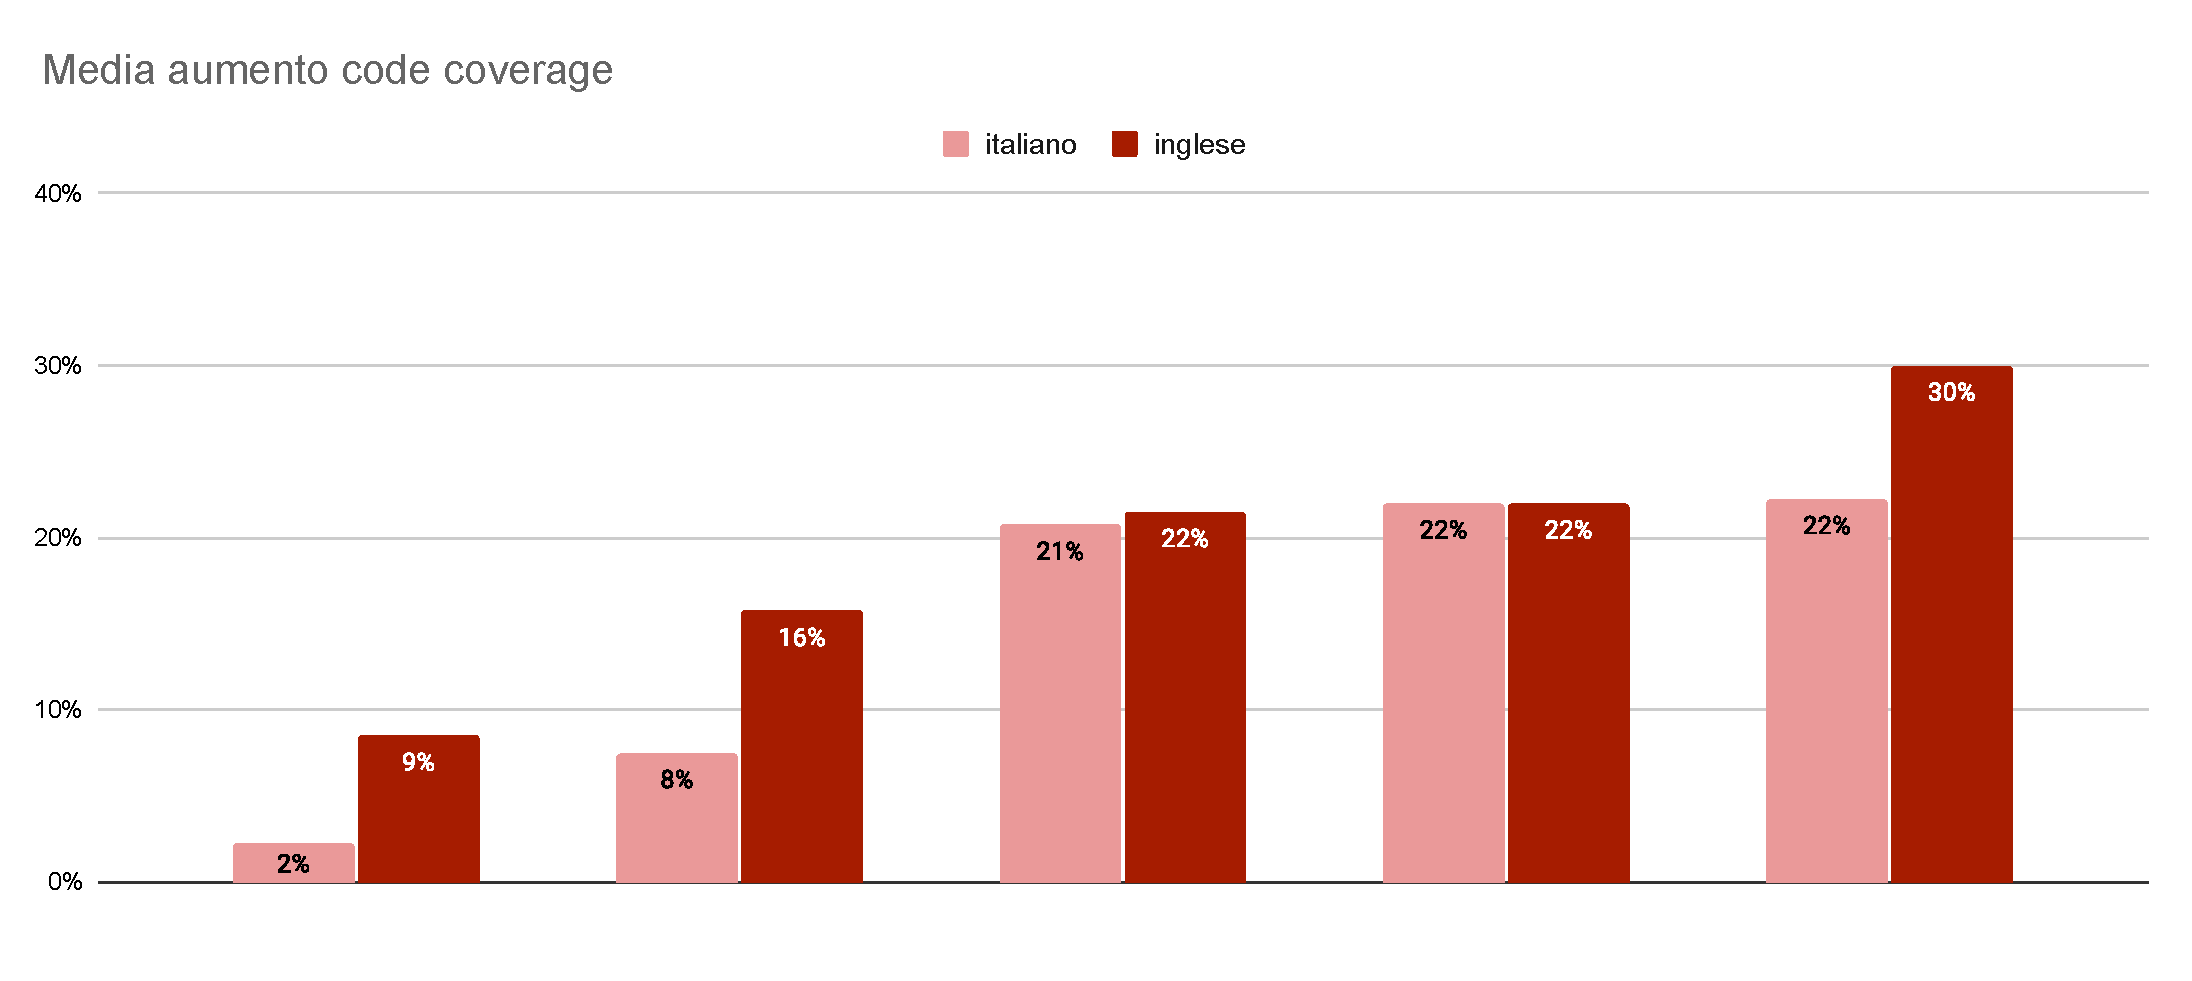
\includegraphics[width=14.5cm]{img/Media aumento code coverage.pdf}
        \caption{Media degli aumenti del code coverage al variare della lingua}
    \end{figure}\newpage
    In figura 3.7 notiamo invece che la media degli aumenti del \textit{code coverage} è sempre maggiore per le richieste su codice sorgente in inglese rispetto a quelle in italiano.
    L'ipotesi quindi che il codice in inglese possa ottenere risultati migliori rispetto a quello in italiano è confermata.
    \newpage
\section{Resoconto finale}
    In questa sezione si procederà a fornire un resoconto finale del lavoro svolto durante il primo macroperiodo, analizzando i risultati ottenuti e le problematiche affrontate.
    \subsection{Prodotti ottenuti}
    Durante il primo macroperiodo di lavoro sono stati ottenuti diversi risultati, tra cui la realizzazione di uno \textit{script} per l'estrazione e la generazione dei \textit{test} automatici.
    In particolare, lo \textit{script} permette di effettuare il parsing di un intero progetto, salvando i dati chiave all'interno di un database SQLite.
    Questo procedimento consente all'\gls{llm} di individuare le relazioni tra i vari metodi e le classi, facilitando la generazione dei \textit{test}.
    Inoltre, sono stati effettuati diversi \textit{benchmark} per valutare le prestazioni dei vari \gls{llm} utilizzati, confrontando i risultati ottenuti.

        %script python per generare test scegliendo le classi e analizzando i vari llm
        %lista prodotto ottenuto
    \subsection{Risultati ottenuti}
        I risultati ottenuti sono stati più che soddisfacenti. Comprendere l'importanza di avere un linguaggio tipizzato per l'analisi sintattica è stato infatti fondamentale per fornire risultati e constatazioni all'azienda Zucchetti.
        Inoltre, l'esecuzione dei \textit{benchmark} per valutare le prestazioni dei vari \gls{llm} utilizzati è stato un passo fondamentale 
        per capire quale fosse il modello e la tipologia di \textit{prompt} più adatto per un futuro sviluppo. 
        Nonostante il lavoro finora svolto risulti soddisfacente, persistono alcune aree di indagine e miglioramento. 
        Tra queste, si segnala la necessità di affrontare l'incertezza riguardante la correttezza del codice generato, 
        che può essere erroneo e deve essere scartato, oppure evidenziare la presenza di un difetto nel sistema, rendendolo di conseguenza un \textit{test} di rilevanza significativa.
        %\cite{article:Hu2021LoRALA}
        %problematiche relative al fatto che se non applico filtri di LLMSE il modello non è in grado di generare codice sorgente valido
        %ma non so se questo codice non è valido perchè è errato o perchè ha trovato un bug
    \subsection{Conclusione}
        %conclusione di tutto il lavoro svolto quindi prodotto         
        % bene o male, pro e contro del PROGETTO e di come è stato affrontato
        Durante l'implementazione del progetto si sono affrontate diverse sfide, tra cui la complessità dell'analisi sintattica in linguaggi non tipizzati, 
        come nel caso di Python, e la complessità del funzionamento delle reti neurali. Una difficoltà aggiuntiva è stata rappresentata dalla limitatezza delle risorse computazionali disponibili. 
        Anche se lo stage si è svolto in un'azienda di rilievo come Zucchetti, le risorse a disposizione non sono sempre state sufficienti per l'utilizzo di modelli linguistici di grandi dimensioni, 
        come Mixtral 7x8b o Wizardlm-2 8x22b. Inoltre, la natura intricata del progetto e la scarsità di materiale informativo relativo all'argomento \gls{llmse} hanno costituito ulteriori ostacoli. 
        È importante notare che \gls{llmseg} è ancora un argomento in fase embrionale, il che si traduce in una carenza di risorse documentative a riguardo. Nonostante queste sfide, 
        il primo macroperiodo del progetto è stato affrontato con successo, generando risultati significativi e fornendo basi solide per uno sviluppo futuro.